% !TEX root = ../SYSprojektrapport.tex
% SKAL STÅ I TOPPEN AF ALLE FILER FOR AT MASTER-filen KOMPILERES 

\label{Modelopbygning}

\section{Model}

For at undersøge husstandsbatterier indflydelse i et el net er der simuleret 5 byer med ca. 2000 hustande, der alle har et batteri installeret. Hver hustand er sat til at have et gennemsnitligt dagligt forbrug på 14kWh,\footnote{https://orsted.dk/Privat/Faa-en-lavere-regning/Kom-godt-i-gang-og-spar-paa-energien/Test-dit-gennemsnitsforbrug/Elforbrug}. Det giver et gennemsnitlig forbrug på 1183kW per by, og en total gennemsnitlig belastning for modelen på 5914kW. For at finde en maks. belastning, forholdet mellem fossile brændsler og vedvarende energi er der taget udgangspunkt i Energinets belastning og produktions information fra Danmark. Det er undersøgt hvor stor en del den gennemsnitlige belastning i modelen udgør af Danmarks gennemsnitlige belastning og derved fundet en skallerings faktor på 716. Denne skallerings faktor er brugt til at finde en samlede maks. belastning for byerne ved dividere med Danmarks maksimale belastning. Den maksimale belastning for hver by ligger derved på 1524kW.

 
 \begin{figure}[H] % (alternativt [H])
 	\centering
 	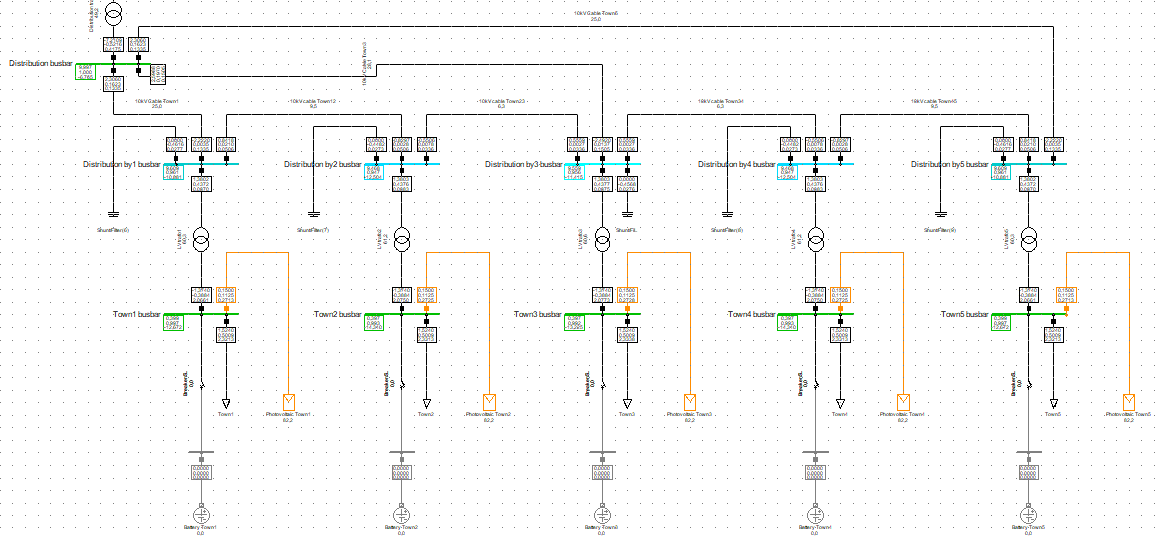
\includegraphics[width=1\textwidth]{figurer/Sim_model_2}
 	\caption{Systemets belastning og distribution}
 	\label{fig:Simdis}
 \end{figure}
    



\begin{figure}[H] % (alternativt [H])
	\centering
	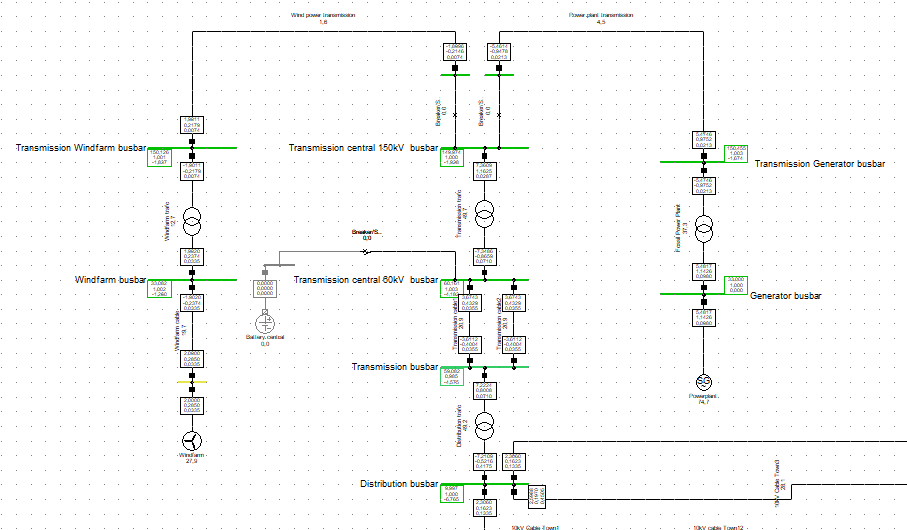
\includegraphics[width=1\textwidth]{figurer/Sim_model_1}
	\caption{systemets produktion transmission}
	\label{fig:SimTrans}
\end{figure}
